\section{System}
We design the proposed system with modularity in mind


\begin{figure*}[t]
\centering
\vspace{-2mm}
 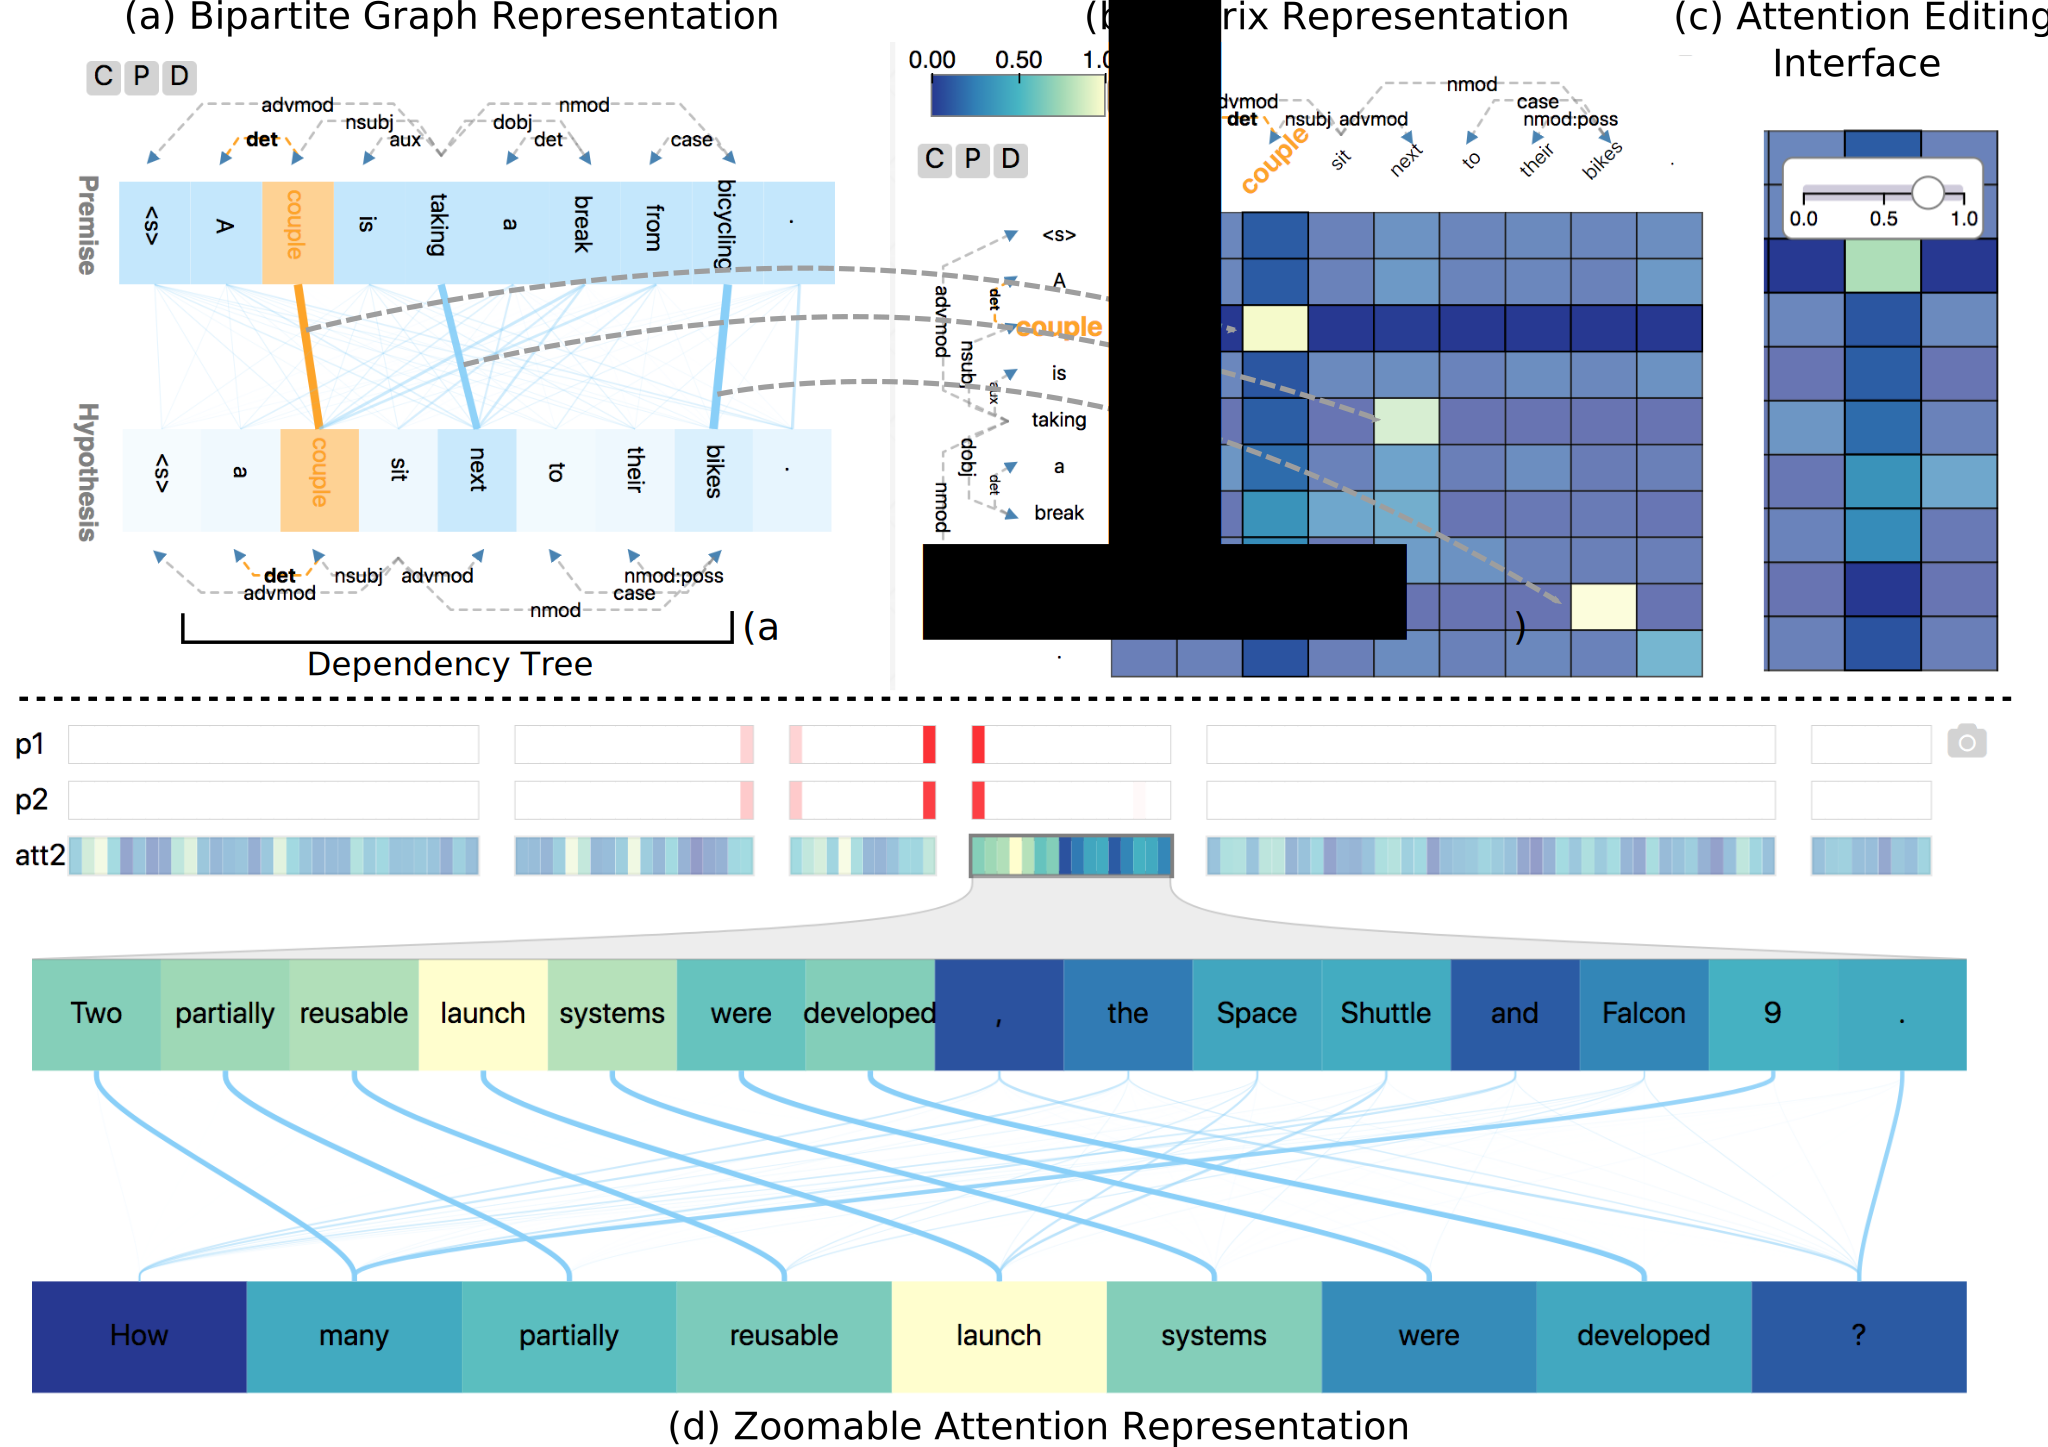
\includegraphics[width=1.0\linewidth]{attentionPanels}
  \vspace{-6mm}
 \caption{
Attention visualization. In the graph attention view (a), a bipartite graph encoding is adopted, in which the edge thickness corresponds to the attention value. In the matrix attention view (b), the entries of $i^{th}$ row represent the probabilities of words in hypotheses align to the $i^{th}$ word in the premise.
The user can alter the attention values via the pop-up interface illustrated in (c).
We overlay the dependency tree ($a_1$) grammar structure to highlight important words and allow simplification of complex sentence based on the dependency tree.
%
For highly asymmetric attention relationship, we utilized a zoomable hierarchical visual representation (d).
}
\label{fig:attention}
\end{figure*}

\subsection{Attention Views}
As illustrated in Figure~\ref{fig:attention}(a)(b), the most widely adopted technique to bipartie graph

Attention matrix


\subsection{Perturbation based exploration}
\label{sec:perturb}

\subsection{Prediction Summarization}



